\documentclass[bachelor]{njupthesis}

\title{定向覆盖模糊测试工具的设计与实现}
\author{雷尚远}
\advisor{王子元}
\school{计算机学院、软件学院、网络空间安全学院}
\major{计算机科学与技术}
\studentclass{B190303}
\studentid{B19030334}
\graduateyear{2023}
\begindate{2023年3月x日}
\finishdate{2023年6月x日}


\begin{document}

\makecover

\begin{chineseabstract}
模糊测试(Fuzzing)是一种通过向目标系统提供非预期的输入并监视异常结果来发现软件安全漏洞的方法,
是软件安全领域常用的方法之一。由于代码覆盖率与漏洞覆盖率密切相关,大多数模糊测试工具都是
以代码覆盖率为导向。然而,由于大多数被覆盖测试的代码可能并不包含漏洞,这使得盲目地扩展
代码覆盖率的方式在实际测试时效率较低。极端情况尤为如此。与盲目增加代码覆盖率的模糊测试不同,
定向覆盖的灰盒模糊测试(DGF)将大部分时间用于检测特定目标区域(例如,易出错代码段)而不会
浪费资源于不相关的部分。因此,DGF 特别适用于补丁测试、漏洞复现以及特殊漏洞检测等场景。
目前,DGF 已成为一个快速发展的研究方向。基于一些先进的定向覆盖模糊测试工具的研究和相关调查,本文
主要做了以下点工作:
\begin{enumerate}[label=(\arabic*)]
	\item 基于现有的模糊测试工具框架AFL(American Fuzzy Lop)以及AFLGo做了定向覆盖策略的设计和集成;
	\item 实现了简单的定向覆盖的模糊测试命令行工具;
	\item 针对相应的公开通用漏洞集(CVE)做了复现及定向实验对比测试。
\end{enumerate}
此外本文亦通过分析工具设计以及实现过程中的局限性与不足,对于未来该方向的研究发展做出了一些展望。

\chinesekeyword{模糊测试;定向覆盖模糊测试;灰盒测试;软件安全}
\end{chineseabstract}

\begin{englishabstract}
Fuzzing is a method of discovering software security vulnerabilities by providing 
unexpected inputs to a target system and monitoring for abnormal results. It is one of the 
commonly used methods in the field of software security. As code coverage is closely related 
to vulnerability coverage, most fuzz testing tools are guided by code coverage. However, blindly 
extending code coverage may be inefficient in practical testing since most of the covered code 
may not contain vulnerabilities, especially for corner cases.  In contrast to blind code coverage-based 
fuzz testing, directed grey-box fuzzing (DGF) spends most of its time detecting specific target regions 
(such as error-prone code segments) rather than wasting resources on irrelevant parts. 
Thus, DGF is particularly suitable for scenarios such as patch testing, bug reproduction, and 
special bug detection. For now, DGF has become a fast-growing research area.  Based on some advanced 
directed coverage fuzz testing tools and relevant investigations, this article mainly focuses on the 
following points of work:
\begin{enumerate}[label=(\arabic*)]
	\item Designed and integrated a directed coverage strategy based on the existing fuzzy testing tool framework AFL (American Fuzzy Lop) and AFLGo;
	\item Implemented a simple command-line tool for directed fuzz testing;
	\item conducted reproductions and directed experiments on corresponding public vulnerability databases (CVE) for comparative testing。
\end{enumerate}
In addition, this article also provides some prospects for the future research and development of this direction by 
analyzing the limitations and deficiencies in the design and implementation process of the tool.


\englishkeyword{Fuzzing;Directed Greybox Fuzzing;Greybox test;Software Security}
\end{englishabstract}

\thesistableofcontents

\thesischapterexordium

\chapter{绪论}
\section{背景分析}
“常用系统中可能会潜伏着严重的漏洞\cite{miller1990empirical}。”这一论述源自于模糊测试首次面世的论文。其
揭示了一个事实,即随着软件技术的不断发展,软件安全问题就将日益成为愈发重视的议题。在当前的信息化时代,
软件已经成为了人们生活、工作和娱乐的重要组成部分,这也意味着我们将面临着越来越多的安全威胁。
因此,确保软件安全已经成为了一项非常重要的任务。

软件安全(Software Security)就是使软件在受到恶意攻击的情形下依然能够继续正确运行及确保软件被在授权范围
内合法使用的思想。在当今社会,软件越来越普及,并被广泛应用于各个领域,包括电商、金融、医疗等。但是,
由于软件的复杂性和开发过程中的缺陷,软件本身也存在着各种安全问题。这些问题可能导致信息泄露、数据损坏、远程攻击等,
对个人、企业甚至整个社会造成巨大的损失。因此,保障软件安全显得尤为重要。

近年来,因为软件漏洞造成的损失案例屡见不鲜。2017年,全球范围内爆发了 WannaCry 勒索病毒攻击事件,
该攻击利用了微软 Windows 操作系统中的漏洞,并导致了数十亿美元的经济损失;2019年,美国资讯技术服务公司 SolarWinds 
遭受了一次大规模的网络攻击,该攻击利用了 SolarWinds Orion 平台软件中的漏洞,影响了包括
美国联邦政府在内的许多组织和机构;2021年2月,法国LCL银行的客户登录自己的银行应用程序时,
看到的是别人的银行账户信息。原因是由于备份超级计算机系统(日本惠普公司制造)的程序存在缺陷,超级计算机系统出现
了意外,其中存储(/ LARGE0)中的某些数据被误删除;2021年12月,知名日志框架Log4j2被爆出远程代码执行漏洞,
影响了大量使用该框架的中间件和应用,给企业和用户带来了巨大的安全风险。

以上诸多例子可以说明,大多数的安全事件都是攻击者利用软件系统中的漏洞从而进行攻击引发的。因而可以帮助发现和
修复安全漏洞的软件测试技术(Software testing)一直以来都是是软件安全领域的一个重要议题。

软件测试可以通过模拟攻击者的行为来发现这些安全漏洞,并提供关于如何修复这些漏洞的信息。例如,
黑盒测试可以探测应用程序中的安全问题,白盒测试可以评估应用程序的源代码中是否有漏洞,
静态分析可以扫描源代码以发现潜在的安全问题,动态分析可以模拟攻击场景并检查应用程序的反应。

此外,软件测试还可以帮助确保应用程序在面对各种攻击时具有足够的鲁棒性和可靠性。它可以测试应用程序的
身份验证和授权机制、加密技术、网络协议、输入输出数据验证等方面的功能,以确保应用程序满足安全需求。

\section{国内外研究现状}
软件安全信息系统和软件安全代码的有效安全项目往往依靠两种自动的安全测试:静态安全扫描测试和动态安全扫描测试。

在软件的开发期间,为了保证软件的安全性,通常会进行软件安全静态扫描。这个过程是通过威胁建模和分析来完成的,
其目的是对静态代码进行全面地扫描,以便及早地发现任何可能存在的安全漏洞。其是在不运行程序的情况下对软件
进行测试和评估。静态分析可以检查代码、设计和文档等,以发现潜在的问题和错误,并确保软件符合某些标准或规范。由于本文
主要探讨针对代码的漏洞审查,关于软件工程部分的文档、标准以及接口设计的测试技术在此不再赘述。利用数据流分析,符号执行
以及污点分析等静态软件分析技术可以检查源代码中的错误和缺陷,包括语法错误、类型错误、内存泄漏、空指针引用等。
与传统的动态测试相比,静态扫描可以更早地发现安全问题,因为它可以在代码尚未被编译或执行之前就进行检测。
此外,静态扫描还可以减少测试成本,提高测试效率,并帮助开发团队更好地理解代码中的潜在安全风险。

软件安全动态扫描是一种对工作环境中实际运行的代码进行扫描的技术,它能够在代码运行时检测和分析可能存在的漏洞、
缺陷和错误。与静态代码分析不同,动态扫描具有更强的准确性和实时性,因为它是在真实的环境中对代码进行测试和评估。
通过使用动态扫描技术,开发人员和安全专家可以有效地识别并修复潜在的安全漏洞,从而保护软件系统免受攻击和破坏。
此外,动态扫描还可以帮助企业遵循各种合规性标准和法规要求,确保其软件应用程序的安全性和稳定性。

模糊测试技术(Fuzzing)是动态安全扫描测试中重要的一种方式。而自从1988年模糊测试这一概念被提出后,
这一方法一直在软件安全测试领域保持着较高的活跃度和关注度。在提出伊始,其主要用于测试操作系统。之后,随着软件技术的发展,
模糊测试技术不断得到改进和推广,并应用于网络、移动设备等领域。目前,模糊测试技术已成为一种成熟的自动化测试技术,
可以有效地检测软件中存在的漏洞和安全隐患。并且迄今为止其社区依然十分活跃,在GitHub上有超过1000个与模糊测试相关的仓库\cite{manes2019art}。
为了防止被恶意攻击,许多商业软件公司,例如Adobe, Cisco, Google, 和Microsoft都将模糊测试作为其雇员软件开发安全测试的必要环节。
可以说,模糊测试是软件安全领域中一个经久不衰的热门议题。

而定向模糊测试(Directed Fuzzing)作为模糊测试的一个研究方向,主要关注重点区域(例如, 易出错区域) 并且将大
部分的时间用于到达测试这些位置而不浪费资源在无关部分\cite{wang2022}。从本源上讲, 定向模糊测试工具早期的解决思路
主要是基于利用程序分析和约束求解来生成检测不同程序执行路径输入符号的执行技术
\cite{ganesh2009taint,ma2011directed,person2011directed,do2013dynamic,ge2011dyta,li2013software}。
然而, 由于定向符号执行技术(DSE) 依赖于大量的程序分析和约束求解, 其受限于兼容性和可扩展性的限制。

在2017 年, Böhme等人提出的AFLGo\cite{bohmeDGF2017}引入了定向灰盒模糊测试(DGF)的概念。这是定向模糊测试的又一重要工作。
其开创式地将将位置的可达性问题转化为生成种子和其目标集之间距离的最小值问题。通过给更靠近目标集的种子更多的变异机会, 它可
以逐渐引导灰盒测试接近程序目标位置。与定向符号执行技术相比, DGF有更好的可拓展性,并且在测试效率上有几个数量级的提升。
例如, Böhme 等人可以在20 分钟内重现 Heartbleed\cite{Heartbleed}(CVE-2014-0160)漏洞, 而定向符合执行工具
KATCH\cite{marinescu2013katch} 需要24小时以上\cite{bohmeDGF2017}。

此后,许多基于AFLGo的定向性改进工作被相继提出。在2018年,Hongxu Chen等人提出的Hawkeye\cite{chen2018hawkeye}
指出了AFLGo的距离计算方式导致的能量分配偏向导致的在测试的路径选择上偏向于距离目标更近的路径(或最短路径),而这有
可能漏掉一些存在于较长路径上潜在的漏洞,于是其使用了新的距离度量来辅助达到更精确的距离导引;在2020年Wang等人
提出的UAFL\cite{wang2020typestate}开创了针对于特定漏洞行为的定向性导引,其利用目标行
为次序而不是目标位置来查找释放后使用的漏洞,这种漏洞的内存操作一定要按照一定次序执行(例如, 分配,
使用, 然后释放内存) 才能触发;在2021年Gwangmu Lee等人提出的CDGF\cite{lee2021constraint}则
指出AFLGo在路径选择中的不考虑执行路径导致的目标位置的顺序影响从而忽略满足特定行为引起崩溃条件的种子的缺陷,
他们的解决思路不再是利用AFLGo的种子分配能量的方式来指引种子变异从而检测指定目标位置,而改为将其视作约束求解问题,
通过设置一系列的约束来优先考虑选择符合要求的种子从而达到检测指定目标位置的目标;而在2022年由Heqing Huang等人
提出的BEACON\cite{huang2022beacon}则从另一种方式进一步尝试提高定向模糊测试的速率:通过“剪枝”,
即修建无效路径的方式。其结合轻量级的静态程序分析,来计算到达目标位置的抽象前提条件,
并在运行时剪除那些不满足条件的路径,从而可以有效地提高效率,避免在无效或不可达的路径上浪费时间和资源。

\section{研究内容}
首先,针对于模糊测试技术,本文做了一个简单的梳理,对于目前模糊测试的基本主流技术框架做了分析和总结。自1988年这一技术
的提出以来,相关技术研究百花齐放,技术快速迭代发展,直到近些年才有相关的总结研究和谱系分析\cite{manes2019art,zhu2022fuzzing},
建立系统性的分析。本文在参考相关文献的基础上对模糊测试的技术框架做了一个梳理。

其次,针对于定向灰盒模糊测试的开篇之作AFLGo,本文对其的技术架构做了一个详细的总结梳理。对于AFLGo的一些实现细节做了详细的
分析和总结。除此之外,本文还探讨了AFLGo在实际应用中的优缺点以及相比于其他模糊测试工具所具备的特点。
针对AFLGo的优点,我们详细阐述了其灵活性、高效性和可扩展性,同时也分析了其在某些情况下可能会出现的一些问题。
此外,本文还介绍了AFLGo在不同场景下的应用,帮助读者更好地理解如何使用AFLGo进行测试。

最后,参考以AFLGo,Hawkeye为主的定向性模糊测试工具,针对于AFLGo的架构进行了改进和集成。本文主要从距离定义和目标函数集合覆盖
率两个指标针对于定向策略做了设计和修改,并结合定向模糊测试工具AFLGo和LLVM的Pass\cite{Pass}技术做的静态分析的实现,
实现了指标在AFLGo的集成。最终,本文在实现后通过实验成功复现libxm2\cite{Libxml2}的CVE-2017-\{9047,9048\},证实了
集成的可行性和可靠性。

\section{论文结构}
本文共分六章,各个章节的内容如下:

第一章:主要介绍本文的研究背景、国内外研究现状、研究内容以及本文的论文结构。

第二章:主要介绍本文涉及技术的详细定义及通用架构,包括模糊测试技术和定向模糊测试技术,以及介绍利用这些技术的典型测试工具架构,最后阐述本文的研究动机。

第三章:介绍AFLGo的主要架构和适应度指标,以及针对于其不足设计出的定向模糊测试适应度指标。详细阐述相应指标的核心设计,
包括插桩,目标函数集覆盖率的计算。

第四章:结合目标场景对实现的定向模糊测试工具做了需求分析,详细介绍了基于LLVM的Pass技术实现的插桩以及静态分析过程
。对于结构集成以及实现方式的缘由做了详细分析。

第五章:对于实现集成的工具进行了实验测试,并做了相应的测试评估,包括工具测试的可行性和性能评估。

第六章:总结了本文的工作并对于未来定向模糊测试技术的发展及研究方向做了展望。

\chapter{相关技术研究}
\section{模糊测试技术}
模糊测试(Fuzz Testing)是一种软件测试技术,其主要思想是通过向输入参数、文件、网络请求等随机或半随机注入无效、
异常、边界数据,来检测目标系统在处理异常情况时的鲁棒性。模糊测试可以帮助发现那些未经预料的漏洞和错误,
这些问题可能会导致应用程序崩溃、停止响应或者执行意外的操作。

在进行模糊测试时,测试人员通常需要编写一个模糊测试工具,该工具可以生成大量的随机测试用例,并将这些测试用例输入
到应用程序中进行测试。模糊测试通常被认为是一种高效的测试技术,因为它可以在较短的时间内检测应用程序中的许多潜在问题。
此外,由于测试用例是随机生成的,模糊测试可以找出一些没有被其他测试方法发现的漏洞和错误。

模糊测试的过程通常分为以下几个步骤:

\begin{enumerate}[label=(\arabic*)]
	\item 选择目标:选择需要测试的软件目标,如应用程序、库、操作系统等。
	\item 寻找输入:确定需要对目标注入的输入类型和数据源,如输入参数、文件、网络请求等。
	\item 创建模糊数据:使用随机或半随机的方式生成模糊数据,并将其注入到目标中。
	\item 监控程序行为:监控被测试程序的运行行为,如崩溃、错误输出等。
	\item 分析结果:对测试结果进行分析和报告,识别潜在的漏洞和安全问题,并反馈给开发人员进行修复。
\end{enumerate}

模糊测试是一种简单有效的测试方法,可以在较短时间内发现大量的异常情况,并帮助开发人员提高软件质量和安全性。

\subsection{基本概念定义}
为了准确地讨论学界关注的模糊测试方向的问题以及梳理架构,我选择了采用Man{\`e}s等人于论文\cite{manes2019art}中
提出的基本概念的定义。

\begin{itemize}
	\item \textbf{Fuzzing}:模糊测试技术是指使用从超出被测试程序(PUT)的预期输入空间的输入空间(“模糊输入空间”)采样的输入来执行被测试程序。
	 \\ 事实上,模糊输入空间(fuzz input space)在定义中并不一定需要包含预期输入空间,其只需要包含预期输入空间所没有的输入即可;其次,
	 因为在实践中大部分模糊测试几乎必然会选择多次迭代来实现测试,故而上述定义补充为“重复执行”依然很大程度上是准确的;最后,关于对于模糊输入空间
	 的采样并不必然是随机的,这与算法设计的种子优先级排序以及采取的变异方式等实现方式有关,故定义并没有加上“随机采样”。
	 \\ 
	\item \textbf{Fuzz Testing}:模糊测试是指使用模糊测试技术(Fuzzing)来测试被测试程序是否违反正确性策略。
	\\ 在诸多论文\cite{householder2012probability,rebert2014optimizing,bohme2020fuzzing}中依然可以见到另一种说法 --- Fuzz Campaign(模糊测试活动),
	用以指明利用特定的模糊测试工具针对具体的被测试程序的一次实际测试活动,但在本文中不再区分这一概念,统一用模糊测试来做指代。
	\\ 
	\item \textbf{Fuzzer}:模糊测试工具是对被测试程序执行模糊测试的程序。
	\\ 
	\item \textbf{Bug Oracle}:错误检测器是一个程序,可能是模糊测试工具的一部分,它确定被测试程序的给定执行是否违反了特定的正确性策略。
	\\ 执行模糊测试的目标当然是查找被测程序的漏洞。但是不同模糊测试工具设计的针对的软件正确性准则(correctness policy)并不相同。例如,早期的
	模糊测试的主要的准则仅仅是生成的测试用例是否会导致被测程序的崩溃(crash);事实上,以SECFUZZ\cite{tsankov2012secfuzz}为代表的许多测试工具
	就将模糊测试引入了包括网络密钥交换协议等非严格软件安全的领域。一般来讲,任何可以通过实际执行的状况中观察到的策略,都可以通过模糊测试来进行安全测试。
	故而所有确定执行表现是否违反特定的正确性策略的机制部分都可以被称作为错误检测器。在本文中,依然将错误检测器执行的软件正确性准则视为导致被测试软件崩溃,其余
	准则不加以讨论。
	\\ 
	\item \textbf{Fuzz Configuration}:模糊测试算法的配置是指所有能控制模糊测试算法执行的参数配置。
	\\ 出于一般性,在此处将所有能够影响到模糊测试算法执行的参数因子都统一称为算法配置。不同的模糊测试算法关注的参数各不相同。例如,最简单的输入随机生成比特流
	输出至被测试程序的模糊测试工具的配置可能仅仅是被测试程序的状态空间,而复杂的模糊测试算法的配置则可能涉及到算法执行时间,随机输入的结构,随机变异策略,前置静态
	分析结果等等。而一般情况下,最受大家关注的配置就是种子的状况。
	\\ 
	\item \textbf{Seed}:种子是被测试程序的(通常结构良好的)输入,一般用于通过修改它来生成测试用例。
\end{itemize}

\subsection{基本架构}
算法\ref{alg:fuzzing}是一般化的模糊测试算法。现如今的大部分模糊测试工具基本是以此流程架构设计。 
这个算法足够通用且具有一般性,可以代表现如今所有的模糊测试技术,包括黑盒模糊测试,白盒模糊测试以及黑盒模糊测试。

本算法也可以简单提炼为模糊测试算法的五个基本步骤,即为:预处理(preprocessing)、调度(schedule)、输入构造(input genaration)、
输入评估(input evaluation)、配置更新(update)。下面将结合算法分别简单介绍各个阶段。

\begin{algorithm}[H]
	\SetKwSty{algokeywordsty}
	\SetFuncSty{algofuncsty}
	\SetDataSty{algodatasty}
	\SetArgSty{algoargsty}
	\SetCommentSty{algocmtsty}
	\SetKw{break}{break}
	\SetKw{not}{not}
	\SetKwFunction{preprocess}{\textsc{Preprocess}}
	\SetKwFunction{schedule}{\textsc{Schedule}}
	\SetKwFunction{inputGen}{\textsc{InputGen}}
	\SetKwFunction{inputEval}{\textsc{InputEval}}
	\SetKwFunction{confUpdate}{\textsc{ConfUpdate}}
	\SetKwFunction{continue}{\textsc{Continue}}
	\SetKwFunction{isBug}{isBug}
	\SetKwFunction{getProgram}{getProgram}
	\SetKwData{newbugs}{$\bugs^\prime$}
	\KwIn{\confs, \timeout}
	\KwOut{\bugs \tcp{a finite set of bugs}}
	$\bugs \gets \varnothing$\;
	$\confs \gets \preprocess{$\confs$}$\;
	\While {$\currtime < \timeout \land \continue{\confs}$}{
	  \conf $\gets \schedule{\confs, \currtime, \timeout}$\;
	  \testcases $\gets \inputGen{\conf}$\;
	  \tcp{\bugoracle is embedded in a fuzzer}
	  \newbugs, \execinfos $\gets$ \inputEval{\conf, \testcases, \bugoracle}\;
	  $\confs \gets \confUpdate{\confs, \conf, \execinfos}$\;
	  $\bugs \gets \bugs \cup \newbugs$\;
	}
	\Return{\bugs}\;
	\caption[short]{模糊测试算法}\label{alg:fuzzing} 
\end{algorithm} 
\vspace{6pt}
预处理:在算法\ref{alg:fuzzing}的第2行为针对程序输入的算法配置进行预处理。主要是用户通过提供一组模糊测试配置,而后依据
模糊测试算法进行处理从而返回一组可能经过修改的模糊测试配置。由于采取的模糊测试策略不同,预处理的操作也就不同。例如接受可执行
文件的黑盒测试一般不做处理,而白盒测试和灰盒测试可能会依据算法的设置源代码或者二进制代码的插桩,进行控制流图生成,指针分析以及污点分析
等软件分析流程。一些测试工具还会选择对用户提供的种子进行处理,例如预筛选可能多余的种子,对种子进行合并精简化等。此外,一些针对
内核或库文件进行很难直接运行程序进行测试的模糊测试工具可能还会准备加载相应的驱动程序用以提供测试。

调度:在算法\ref{alg:fuzzing}的第4行为针对执行的算法配置进行调度设置。主要是通过更改或者选择特定的算法配置来
决定接下来算法的行为。在此过程一般为处理模糊测试算法中的探索(exploration)与开发(exploitation)问题。
探索问题是指在执行模糊测试中将此次分配的时间用以收集有关每个配置的更准确信息上,以便为未来的决策提供信息;而开发问题是指
将分配的时间用以针对当前被认为会导致更有利结果的配置进行模糊测试。由于实际被测试的程序不同,待测试的目标复杂度不同以及
需要的精确信息的获取难度不同,实际测试中这两阶段的分界线并不是那样的固定和明确。一般算法仅仅是通过设置策略来引导探索
阶段收集特定所需的信息。

输入构造:在算法\ref{alg:fuzzing}的第5行为针对选择的算法配置来生成相应的测试用例。这与采取的模糊测试技术有关,
一般根据此阶段的策略将模糊测试算法分成基于模型(Model-based)的算法和少模型(Model-less)的算法。由于不同的被测
程序对于输入的格式要求不同,故而对于测试用例的构造也有不同的策略。基于模型的模糊测试工具根据给定的模型生成测试用例,
给定模型描述了被测程序可能接受的输入或执行方式,如准确描述输入格式的语法或较不准确的约束条件,
比如标识文件类型的魔术值(magic values)。因此基于模型的算法又被称为生成式(Generation-based),通过输入的模型来指导
生成测试用例,常用于黑盒模糊测试。而少模型的算法则是依据算法伊始被提供的种子来进行变异生成符合条件的测试用例。这种方式
的出现是为了解决基于模型的生成输入效率不高的问题。除此以外,白盒测试技术可能会采取符号执行的方式来辅助生成测试用例。

输入评估:在算法\ref{alg:fuzzing}的第6行为针对生成的输入进行输入执行测试和进行种子评估。这一步会将生成的测试用例输入
被测试程序来测试被测试程序。根据执行生成的执行信息和错误检测器来判断是否触发了被测试程序的异常行为,这一步将为
下一步的配置更新提供反馈信息(对于黑盒测试,一般就是报告程序错误信息)。

配置更新:在算法\ref{alg:fuzzing}的第7行为依据上一步生成得到的执行信息和反馈信息对算法配置信息进行更新。这些变动
将决定和引导接下来的模糊测试算法的行为。对于黑盒测试而言,这一步一般什么也不做。

\subsection{模糊测试技术的分类}
一般学界会将模糊测试技术分为黑盒模糊测试,白盒模糊测试以及灰盒模糊测试。与传统软件测试中的黑盒测试和白盒测试\cite{myers2011art}定义不同,
对于模糊测试技术的分类是依靠模糊测试工具收集信息的数量来决定的\cite{manes2019art}。

一般模糊测试工具会有多种渠道收集信息,但是最主要的途径依然是通过程序的状况来获得。正如一般化算法\ref{alg:fuzzing}中显示
,事实上只有只有算法的第2行和第7行会对算法的配置进行修改。这对应的即是算法的预处理部分和配置更新部分。也即,这两个步骤获取
程序信息的的数量决定了模糊测试工具的种类(或者讲,“颜色”)。
\section{定向模糊测试技术}
\subsection{白盒定向模糊测试技术}
\subsection{灰盒定向模糊测试技术}
\section{研究动机}
\section{本章小结}

\chapter{定向模糊测试策略设计}
\begin{algorithm}[H]
	\DontPrintSemicolon
	\SetKwSty{algokeywordsty}
	\SetFuncSty{algofuncsty}
	\SetDataSty{algodatasty}
	\SetArgSty{algoargsty}
	\SetCommentSty{algocmtsty}
	\SetKw{break}{break}
	\SetKw{not}{not}
	\SetKwFunction{graphextractor}{\textsc{GraphExt}}
	\SetKwFunction{bbdistance}{\textsc{DisCalcu}}  
	\SetKwFunction{select}{\textsc{Dequeue}}
	\SetKwFunction{assinenergy}{\textsc{AssinEnergy}}
	\SetKwFunction{mutation}{\textsc{Mutation}}
	\SetKwFunction{execution}{\textsc{Execution}}
	\SetKwFunction{IsIntersting}{\textsc{IsIntersting}}
	\SetKwFunction{evaluateseed}{\textsc{SeedDis}}
	\SetKwFunction{sortinsert}{Enqueue}
	% \SetKwData{crashseeds}{$\seeds_{\text{\emoji{boom}}}$}
	\SetKwData{crashseeds}{$\seeds^\prime$} 
	\SetKwData{seedqueue}{$\textit{SeedQueue}$}  
	\SetKwData{Graph}{$\textit{Graphs}$}  
	\SetKwData{BBdis}{$\textit{BBdistance}$} 
	\SetKwData{newseed}{$\seed^\prime$}   
	\SetKwData{energy}{$\textit{e}$}
	\SetKwData{trace}{$\textit{trace}$} 
	\SetKwData{distance}{$\textit{distance}$}   
	\KwIn{\seeds\tcp{a finite set of seeds}}
	\KwIn{\targets\tcp{a finite set of targer sits}} 
	\KwOut{\crashseeds \tcp{a finite set of buggy seeds}}
	$\crashseeds\gets \varnothing$\; 
	$\seedqueue \gets \seeds$\;
	\Graph $\gets \graphextractor{\sourcecode}$\;
	\BBdis $\gets \bbdistance{\targets,\Graph}$\;
	\While {$!siganl \land \currtime < \timeout$}{
	  \seed$\gets \select{\seedqueue}$\;
	  $\trace \gets \execution{\seed}$\; 
	  $\distance \gets \evaluateseed{\trace, \BBdis} $\;
	  \energy $\gets \assinenergy{\seed, \currtime, \distance}$\;
	   \For{$\textit{i}\gets 1$ \KwTo $\energy$}
	   {
		$\newseed \gets \mutation{\seed}$\;      
		\lIf{\newseed crashes}{$\crashseeds \gets \crashseeds \cup \newseed $}
		\lIf{\IsIntersting{\newseed}}{    
			$\sortinsert{\newseed,\seedqueue} $ 
		}
	   }
	}
	\Return{\crashseeds}\;
	\caption[short]{定向灰盒模糊测试算法}\label{alg:DGF} 
\end{algorithm} 
\section{AFLGo架构研究}
\subsection{距离计算机制}
\subsection{能量调度机制}
\section{定向适应度指标}
\subsection{距离定义}
\subsection{目标函数集覆盖率}
\subsection{能量调度机制}
\section{本章小结}


\chapter{基于AFLGo的定向模糊测试系统的实现}
\section{需求分析}
\section{架构设计}
\section{静态分析器的改进}
\section{定向模糊测试工具}
\section{本章小结}

\chapter{系统测试}
\section{系统测试概述}
\subsection{系统测试目标}
\subsection{系统测试环境}
\section{功能测试}
\section{实验评估}
\subsection{定向模糊测试工具}
\section{本章小结}


\chapter{总结与展望}
\section{总结}
\section{展望}

% \section{Apple M1}
% 这是一个公式
% \begin{equation}
% 	y=A x+b
% \end{equation}


% 南京南站如图\ref{南京南站}所示。
% \begin{figure}[hbt]
% 	\centering
% 	\subfigure[南京南1]{
% 		\begin{minipage}[b]{0.4\textwidth}
% 			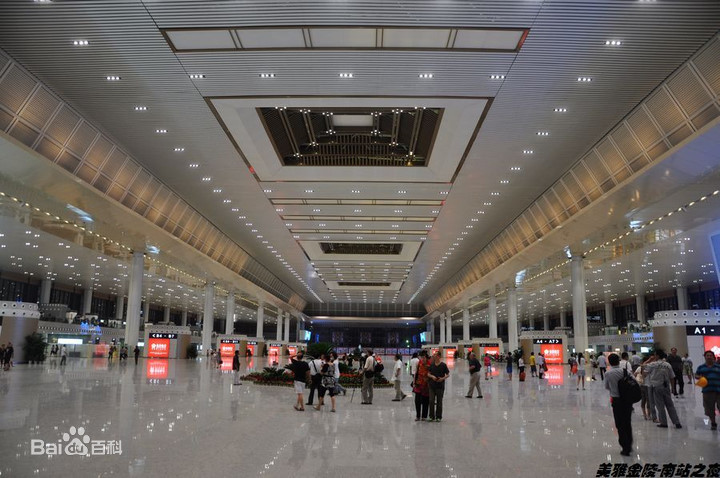
\includegraphics[width=1\textwidth]{1}
% 		\end{minipage}
% 	}
% 	\subfigure[南京南2]{
% 		\begin{minipage}[b]{0.4\textwidth}
% 			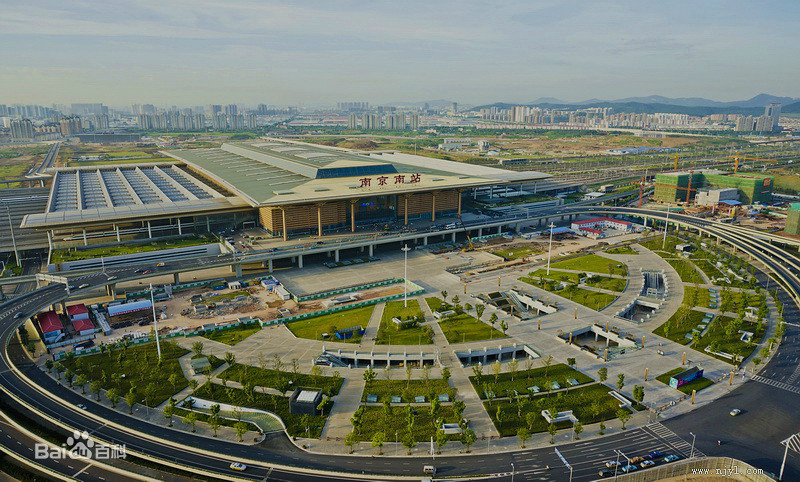
\includegraphics[width=1\textwidth]{2}
			
% 		\end{minipage}
% 	} \\
% 	\subfigure[南京南3]{
% 		\begin{minipage}[b]{0.4\textwidth}
% 			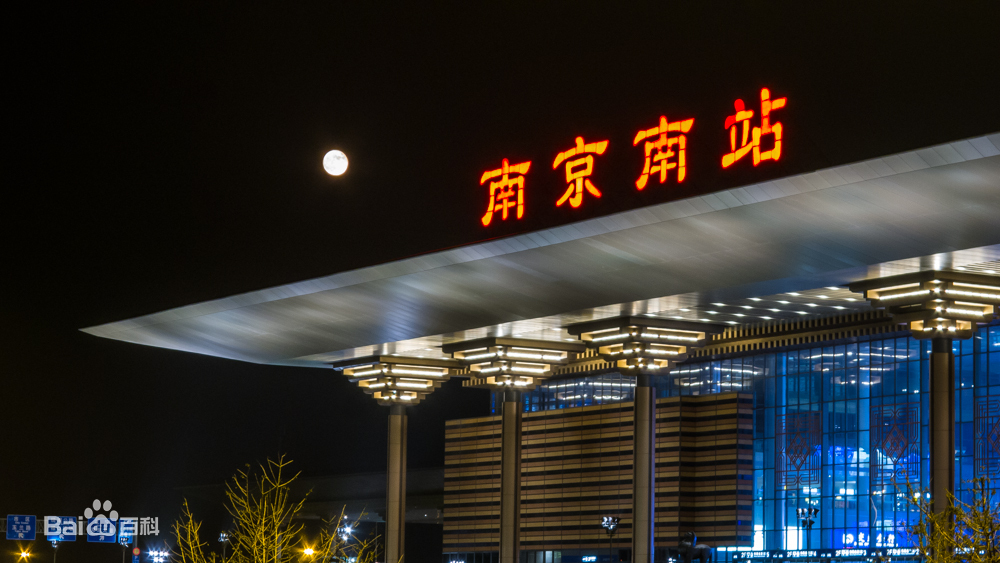
\includegraphics[width=1\textwidth]{3}
% 		\end{minipage}
% 	}
% 	\subfigure[南京南4]{
% 		\begin{minipage}[b]{0.4\textwidth}
% 			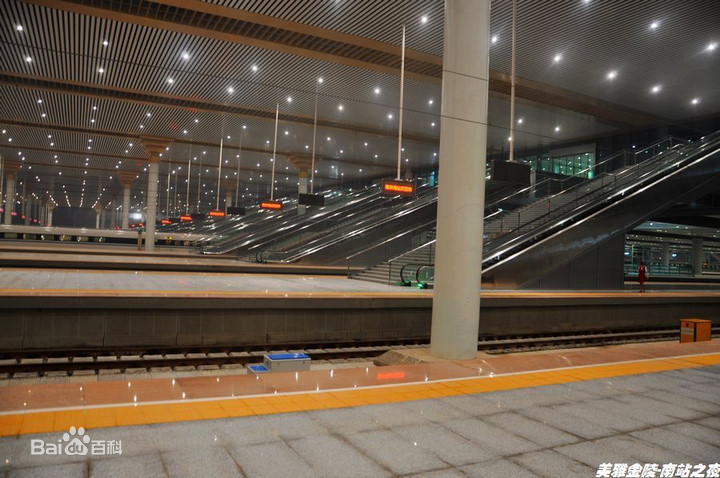
\includegraphics[width=1\textwidth]{4}
			
% 		\end{minipage}
% 	}
% 	\caption{南京南站}
% 	\label{南京南站}
% \end{figure}

%这里是结束语
\thesisconclusion

% 致谢区域
\thesisacknowledgement

本论文采用\LaTeX 模版编写的,是基于南京邮电大学2021年理工艺教类的Word模板进行严格迁移编写的。本模板地址\url{https://github.com/dhiyu/NJUPT-Bachelor}感谢imguozr(\url{https://github.com/imguozr/NJUPThesis-Bachelor} )和lemoxiao(\url{https://github.com/lemoxiao/NJUPThesis-Scholar} )的工作,为本模板的形成奠定了大量的基础。

% 参考文献区域
\thesisreference

\end{document}